\section{Тема 2}

% Множества
\bu{Множество} е първично понятие, което не се дефинира. Интуитивно го определяме като колекция от
различни обекти. Обикновено, но не винаги, имената на множествата са главни латински букви: \(A, B, ...\).
При изреждане на елементите се ползват фигурните скоби \{  \}, а имената на елементите са разделени със
запетаи, например \mexpr{A = \{a, b, c\}}.

Принадлежността към множество се бележи с '\(\in\)', а непринадлежността с '\(\not \in\)', например
\mexpr{a \in \{a, b, c\}; d \not \in \{a, b, c\}}.

Множества може да са елементи на други множества.

\subsection{Аксиома за обема}
Две множества са равни \totw съдържат едни и същи елементи, т.е. 
\mexpr{\forall X \forall Y(\forall z(z \in X \iff z \in Y) \to X = Y)}. \\

От аксиомата за обема следва, че редът в който са записани елементите на дадено множество, както и 
наличието на повторения на елементи, е без значение.
Например: \mexpr{\{a, b, c\} = \{a, a, b, b, b, c\} = \{a, b, c, b, a\} = \{c, b, a\}}.

\subsection{Аксиома за отделянето}
С предикат може да отделим подмножество от множество. \\

Ако \(X\) е множество и \(\pi\) е предикат с домейн \(X\), то съвкупността \(Y\) от елементите на \(X\), които
имат свойството \(\pi\), е множество: \\
\mexpr{\forall X \exists Y \forall z(z \in Y \iff \pi(z))}

Нека \(X\) е множество, \(\pi\) е предикат над него и \mexpr{Y = \{x \in X : \pi(x)\}}. \\
Казваме, че \(Y\) е \bu{подмножество (надмножество)} на \(X\) и пишем \mexpr{Y \subseteq X (X \supseteq Y)}. \\
Имаме следните 2 случая:
\begin{itemize}
    \item \mexpr{\forall x \in X: \pi(x)} \\
    Тогава \(Y = X\). Виждаме, че всяко множество е подмножество на себе си.
    \item \mexpr{\lnot \exists x \in X: \pi(x) \equiv \forall x \in X : \lnot \pi(x)} \\
    Тогава \(Y\) е празното множество. Пишем \(Y = \emptyset\). Празното множество е подмножество на всяко
    множество, включително и на себе си.
\end{itemize}

Когато \mexpr{Y \subseteq X} (\mexpr{X \supseteq} Y), но \mexpr{Y \ne X} казваме, че \(Y\) е \\ 
\bu{същинско подмножество (надмножество)} на \(X\) и пишем \mexpr{Y \subset X (X \supset Y)}, което 
за да бъде изпълнено, трябва да съществува елемент \(x \in X\), такъв че \(x \not \in Y\). 

\subsection{Аксиома за степенното множество}
За всяко множество \(X\) съществува множеството от всички негови подмножества, което наричаме 
степенното множество на \(X\), т.е. \\
\mexpr{\forall X \exists Y \forall z (z \in Y \iff z \subseteq X)}. \\
Бележем го с \(2^X\).

Примери:
\begin{itemize}
    \item \mexpr{X = \emptyset \implies 2^X = \{\emptyset, \emptyset\} = \{\emptyset\}}
    \item \mexpr{X = \{a, b, c\} \implies 2^X = \{\emptyset, \{a\}, \{b\}, \{c\}, \{a, b\}, \{a, c\}, \{b, c\}, \{a, b, c\}\}
\end{itemize}

\subsection{Минималност и максималност по включване}
Нека е дадено множество \(A\) и предикат \(\sigma\) върху \(2^A\).
За всяко множество \mexpr{B \subset A}, казваме, че \(B\) е максимално [минимално] по включване по 
отношение на \(\sigma\), ако:
\begin{enumerate}
    \item \(\sigma(B)\)
    \item \mexpr{\forall C: (B \subset C \subseteq A \to \lnot \sigma(C))} [\mexpr{\forall C: (C \subset B \to \lnot \sigma(C))}]
\end{enumerate}

Максимално [минимално] по включване подмножество е такова, за което предикатът е в сила, но той не е в сила
за никое негово същинско надмножество [подмножество].

За да говорим за максималност и минималност по включване, трябва да имаме предвид предикат. Без предикат,
тези понятия нямат смисъл. \\

Пример: разграничение между "максимално по включване" (maximal) и "глобално максимално" (maximum) чрез клика в граф \\

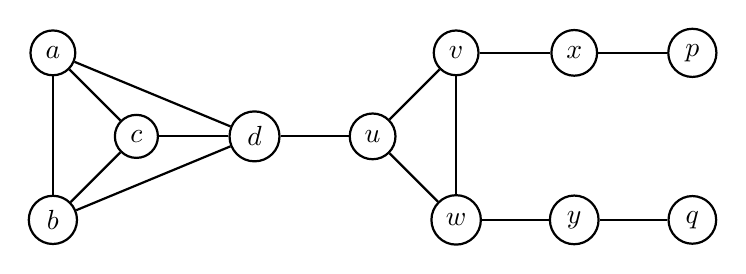
\begin{tikzpicture}[node distance={15mm}, thick, main/.style = {draw, circle}] 
\node[main] (1) {$a$}; 
\node[main] (3) [below right of=1] {$c$};
\node[main] (2) [below left of=3] {$b$};
\node[main] (4) [right of=3] {$d$};
\node[main] (5) [right of=4] {$u$};
\node[main] (6) [below right of=5] {$w$};
\node[main] (7) [above right of=5] {$v$};
\node[main] (8) [right of=7] {$x$};
\node[main] (9) [right of=8] {$p$};
\node[main] (10) [right of=6] {$y$};
\node[main] (11) [right of=10] {$q$};
\draw (1) -- (2);
\draw (1) -- (3);
\draw (1) -- (4);
\draw (2) -- (3);
\draw (2) -- (4);
\draw (3) -- (4);
\draw (4) -- (5);
\draw (5) -- (6);
\draw (5) -- (7);
\draw (6) -- (7);
\draw (7) -- (8);
\draw (8) -- (9);
\draw (6) -- (10);
\draw (10) -- (11);
\end{tikzpicture}

Клика в граф е множество от върхове, всеки два от които са свързани с ребро. \\
Всеки връх е тривиална клика. \\
Примерни клики са \mexpr{\{x, p\}, \{v, x\}, \{u, v, w\}, \{a, b, c, d\}}. \\
Тук \mexpr{\{a, b, c, d\}} е най-голямата клика (т.е. максимална клика - отговаря на "глобално максимално") - 
друга клика с 4 върха няма. Към \mexpr{\{u, v, w\}} не може да се добави връх, запазвайки свойството 
множеството да е клика, т.е. \mexpr{\{u, v, w\}} отговаря на "максимално по включване".

\subsection{Операции върху множества}
Нека \(X\) и \(Y\) са множества.

\begin{itemize}
    \item Обеденението на \(X\) и \(Y\) е \mexpr{X \cup Y =  \{x | x \in X \vee x \in Y\}}.
    \item Сечението на \(X\) и \(Y\) е \mexpr{X \cap Y =  \{x | x \in X \land x \in Y\}}.
    \item Разликата \(X\) и \(Y\) е \mexpr{X \setminus Y =  \{x | x \in X \land x \not \in Y\}}.
    \item Симетричната разлика то на \(X\) и \(Y\) е \mexpr{X \Delta Y =  \{x | x \in X \oplus x \in Y\}}.
    \item Допълнението на \(X\) до даден универсум \(U\) е \mexpr{\overline{X^{U}} =  \{x | x \in U \land x \in X\}}.
\end{itemize}

\subsection{Основни свойства на операциите върху множества}
Нека \(X\), \(Y\) и \(Z\) са множества и \(U\) е универсум.

\begin{enumerate}
    \item Свойство на константите
        \begin{itemize}
            \item \mexpr{X \cup \emptyset = X}
            \item \mexpr{X \cup U = U}
            \item \mexpr{X \cap \emptyset = \emptyset}
            \item \mexpr{X \cap U = X}
        \end{itemize}
    \item Свойство на отрицанието
        \begin{itemize}
            \item \mexpr{X \cup \overline{X} = U}
            \item \mexpr{X \cap \overline{X} = \emptyset}
        \end{itemize}
    \item Идемпотентност
        \begin{itemize}
            \item \mexpr{X \cup X = X}
            \item \mexpr{X \cap X = X}
        \end{itemize}
    \item Закон за двойното отрицание
        \begin{itemize}
            \item \mexpr{\overline{\overline{X}} = X}
        \end{itemize}
    \item Комутативност
        \begin{itemize}
            \item \mexpr{X \cup Y = Y \cup X}
            \item \mexpr{X \cap Y = Y \cap X}
            \item \mexpr{X \Delta Y = Y \Delta X}
            \item \mexpr{X \setminus Y \ne Y \setminus X}
        \end{itemize}
    \item Асоциативност
        \begin{itemize}
            \item \mexpr{X \cup (Y \cup Z) = (X \cup Y) \cup Z = X \cup Y \cup Z}
            \item \mexpr{X \cap (Y \cap Z) = (X \cap Y) \cap Z = X \cap Y \cap Z}
        \end{itemize}
    \item Дистрибутивност
        \begin{itemize}
            \item \mexpr{X \cap (Y \cup Z) = (X \cap Y) \cup (X \cap Z)}
            \item \mexpr{X \cup (Y \cap Z) = (X \cup Y) \cap (X \cup Z)}
        \end{itemize}
    \item Закони на де Морган
        \begin{itemize}
            \item \mexpr{\overline{X \cup Y} = \overline{X} \cap \overline{Y}}
            \item \mexpr{\overline{X \cap Y} = \overline{X} \cup \overline{Y}}
        \end{itemize}
    \item Закон за поглъщането
        \begin{itemize}
            \item \mexpr{X \cup (X \cap Y) = X}
            \item \mexpr{X \cap (X \cup Y) = X}
        \end{itemize}
    \item Свойство на импликацията
        \begin{itemize}
            \item \mexpr{p \rightarrow q \equiv \lnot p \vee q}
        \end{itemize}
    \item Свойство на би-импликацията
        \begin{itemize}
            \item \mexpr{X \subseteq Y \land Y \subseteq X \iff X = Y}
        \end{itemize}
\end{enumerate}

\subsection{Покриване и разбиване на множество}

\boxt{Определение} \\
\bu{Протоелементите} са първични елементи, не са множества. Множествата изграждаме от протоелементи и/или
други множества. \\
Множеството от протоелементите, които може да се появяват, се нарича \bu{опорно множество}. \\
Множество от множества се нарича \bu{фамилия}. \\

Пример: \mexpr{A = \{a, b, c\}} е опорно множество, а фамилии над него са \mexpr{X = \{\{a, b\}, \{c\}\}, Y = \{\{a, c\}\}}

Нека \(X\) е непразно множество. \bu{Покриване} на \(X\) е всяка фамилия \mexpr{X = \{X_1, X_2, ..., X_k\}}
такава, че \(k \ge 1\) и:
\begin{enumerate}
    \item \mexpr{\forall i \in \{1, 2, ..., k\}: X_i \subseteq X}
    \item \mexpr{\forall i \in \{1, 2, ..., k\}: X_i \ne \emptyset}
    \item \mexpr{\cup_{i = 1}^{k} X_i = X}
\end{enumerate}
Ако освен това е вярно и \mexpr{\forall i \forall j (1 \le i < j \le k \to X_i \cap X_j = \emptyset)} казваме, 
че \(X\) е \bu{разбиване} на \(X\).

Пример: нека \mexpr{X = \{x, y, z, t\}}, покриване на \(X\) е \mexpr{\{\{x, y\}, \{y, z, t\}, \{x, z, t\}\}},
разбиване на \(X\) е \mexpr{\{\{x, z\}, \{y\}, \{t\}\}}.

\subsection{Диаграми на Venn}

В пълните диаграми на Venn, универсумът винаги присъства.
Районите са точно \(2^n\) при \(n\) множества.

Общо положение при две множества:

% To add the universum letter U in some corner of the box
% TODO: symetric difference and addition of set

\fbox{
    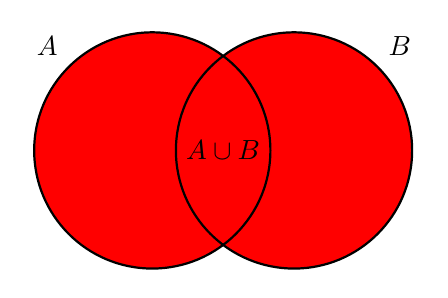
\begin{tikzpicture}[thick,
        set/.style = {circle,
            fill=red,
            minimum size =3cm
        }]
    
    % Set A
    \node [set,
        label={135:$A$}] (A) at (0,0){};
    
    % Set B
    \node [set,
        label={45:$B$}] (B) at (1.8,0){};
    
    % Circles outline
    \draw[black] (0, 0) circle(1.5cm);
    \draw[black] (1.8, 0) circle(1.5cm);
    
    % Union text label
    \node at (0.9, 0) {$A\cup B$};
    
    \end{tikzpicture}}

\fbox{
    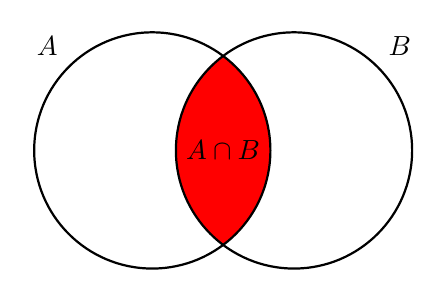
\begin{tikzpicture}[thick,
        set/.style = {circle,
            minimum size = 3cm,
            fill=white}]

        % Set A
        \node[set, label={135:$A$}] (A) at (0,0) {};
        
        % Set B
        \node[set, label={45:$B$}] (B) at (1.8,0) {};
        
        % Intersection
        \begin{scope}
            \clip (0,0) circle(1.5cm);
            \clip (1.8,0) circle(1.5cm);
            \fill[red](0,0) circle(1.5cm);
        \end{scope}
        
        % Circles outline
        \draw (0,0) circle(1.5cm);
        \draw (1.8,0) circle(1.5cm);
        
        % Set intersection label
        \node at (0.9,0) {$A \cap B$};
    
    \end{tikzpicture}}

\fbox{
    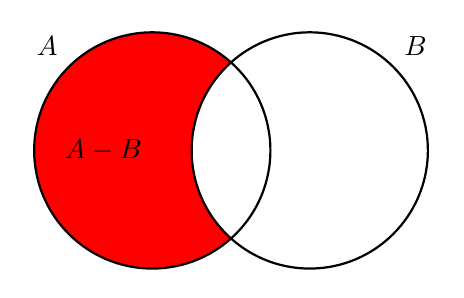
\begin{tikzpicture}[thick,
        set/.style = { circle, minimum size = 3cm}]
    
    % Set A
    \node[set, fill=red, label={135:$A$}] (A) at (0,0) {};
    
    % Set B
    \node[set, fill=white, label={45:$B$}] (B) at (0:2) {};
    
    % Circles outline
    \draw (0,0) circle(1.5cm);
    \draw (2,0) circle(1.5cm);
    
    % Difference text label
    \node[left, black] at (A.center){$A - B$};
    
    \end{tikzpicture}
}

\fbox{
    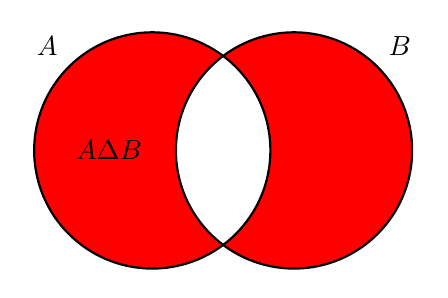
\begin{tikzpicture}[thick,
        set/.style = {circle,
            minimum size = 3cm,
            fill=red}]
     
    % Set A
    \node[set, label={135:$A$}] (A) at (0,0) {};
     
    % Set B
    \node[set, label={45:$B$}] (B) at (1.8,0) {};
     
    % Intersection
    \begin{scope}
        \clip (0,0) circle(1.5cm);
        \clip (1.8,0) circle(1.5cm);
        \fill[white](0,0) circle(1.5cm);
    \end{scope}
     
    % Circles outline
    \draw (0, 0) circle(1.5cm);
    \draw (1.8, 0) circle(1.5cm);
     
    % Set intersection label
    \node[left] at (A.center) {$A \Delta B$};
     
    \end{tikzpicture}
}

\begin{tikzpicture}
    \draw [fill=red] (10, 0) rectangle ++(5, 3);
    \node at (12.5, 1.5) {
        \begin{tikzpicture}
            \draw [fill=white] circle (1cm);
        \end{tikzpicture}
    };
\end{tikzpicture}
